\documentclass[10pt]{article}
\usepackage[ngerman]{babel}
\usepackage[utf8]{inputenc}
\usepackage[T1]{fontenc}
\usepackage{amsmath}
\usepackage{amsfonts}
\usepackage{amssymb}
\usepackage[version=4]{mhchem}
\usepackage{stmaryrd}
\usepackage{bbold}
\usepackage{graphicx}
\usepackage[export]{adjustbox}
\graphicspath{ {./images/} }

\begin{document}
\section*{Diskrete Wahrscheinlichkeitsräume}
\section*{Definition}
Der Ergebnisraum $\Omega$ ist die Menge aller möglichen Ergebnisse des betrachteten Zufallsexperiments.\\
Die Zähldichte ist eine Funktion $\rho: \Omega \rightarrow[0,1]$, die jedem Ergebnis seine Wahrscheinlichkeit zuordnet. Sie wird graphisch als Stabdiagramm dargestellt. Es gilt: $1=\sum_{\omega \in \Omega} \rho(\omega)$.

Ein Ereignis ist eine Teilmenge von $\Omega$; der Ereignisraum $2^{\Omega}$ ist die Menge aller Teilmengen von $\Omega$.\\
Jede Zähldichte bestimmt ein diskretes Wahrscheinlichkeitsmass $P: 2^{\Omega} \rightarrow[0,1], P(M)=\sum_{\omega \in M} \rho(\omega)$ für $M \subseteq \Omega$; dieses ordnet jedem Ereignis seine Wahrscheinlichkeit zu.

Der Ergebnisraum $\Omega$ versehen mit dem Wahrscheinlichkeitsmass $P$ heisst dann diskreter Wahrscheinlichkeitsraum und wird mit $(\Omega, P)$ bezeichnet.

Falls jedes Ergebnis aus $\Omega$ gleichwahrscheinlich ist, wird $(\Omega, P)$ Laplace-Raum genannt. Für diesen Spezialfall gilt: $P(M)=\frac{|M|}{|\Omega|}$.

\section*{Wichtige Eigenschaften diskreter Wahrscheinlichkeitsräume $(\Omega, P)$}
(A1) (Unmögliches Ereignis) $P(\})=0$\\
(A2) (Sicheres Ereignis) $P(\Omega)=1$\\
(A3) (Komplementäres Ereignis) $P(\Omega \backslash A)=1-P(A)$\\
(A4) (Vereinigung) $P(A \cup B)=P(A)+P(B)-P(A \cap B)$\\
(A5) (Sigma-Additivität) $P\left(A_{1} \cup A_{2} \cup A_{3} \cup \ldots\right)=P\left(A_{1}\right)+P\left(A_{2}\right)+P\left(A_{3}\right)+\ldots$\\
falls die Ereignisse $A_{1}, A_{2}, A_{3}, \ldots$ paarweise disjunkt sind.

\section*{Zufallsvariablen}
\section*{Definitionen}
Sei $(\Omega, P)$ ein diskreter Wahrscheinlichkeitsraum.\\
Jede Funktion $X: \Omega \rightarrow \mathbb{R}$, welche auf dem Ergebnisraum definiert ist und reelle Werte hat, heisst Zufallsvariable.\\
Die reelle Funktion $f: \mathbb{R} \rightarrow[0,1], f(x)=P(X=x)$ heisst Wahrscheinlichkeitsdichte oder kurz Dichtefunktion (PMF) von $X$.\\
Die reelle Funktion $F: \mathbb{R} \rightarrow[0,1], F(x)=P(X \leq x)$ heisst kumulative Verteilungsfunktion (CDF) von $X$.

\section*{Wichtige Eigenschaften von PMF und CDF}
(1) $\sum_{x=-\infty}^{\infty} f(x)=1$ und $F(z)=\sum_{x=-\infty}^{z} f(x)$\\
(2) $\lim _{x \rightarrow \infty} F(x)=1$ und $\lim _{x \rightarrow-\infty} F(x)=0$\\
(3) Monotonie: Aus $x \leq y$ folgt $F(x) \leq F(y)$\\
(4) $f(x)=F(x)-\lim _{y \rightarrow x^{-}} F(y)$\\
(5) $P(a<X \leq b)=F(b)-F(a)$ und $P(a \leq X \leq b)=F(b)-\lim _{x \rightarrow a^{-}} F(x)$\\
(6) $P(X>b)=1-F(b)$ und $P(X \geq b)=1-\lim _{x \rightarrow b^{-}} F(x)$

\section*{Kenngrössen}
Um Verteilungen vergleichen zu können bedient man sich einiger weniger charakteristischer Merkmale, sogenannter Kenngrössen. Wir betrachten Lagemasse und Streumasse. Lagemasse beschreiben das Zentrum der Verteilung und Streumasse charakterisieren die Abweichung vom Zentrum.

\section*{Definitionen}
Seien $(\Omega, P)$ ein diskreter Wahrscheinlichkeitsraum und $X: \Omega \rightarrow \mathbb{R}$ eine Zufallsvariable.\\
(1) Der Erwartungswert $E(X)=\sum_{x \in \mathbb{R}} P(X=x) \cdot x=\sum_{\omega \in \Omega} P(\{\omega\}) \cdot X(\omega)$ ist ein Lagemass der Verteilung von $X$. Der Erwartungswert existiert nicht für jede Verteilung.\\
(2) Die Varianz $V(X)=E\left([X-E(X)]^{2}\right)=\sum_{x \in \mathbb{R}} P(X=x) \cdot[x-E(X)]^{2}=\sum_{\omega \in \Omega} P(\{\omega\}) \cdot[X(\omega)-E(X)]^{2}$ und die Standardabweichung $S(X)=\sqrt{V(X)}$ sind Streumasse der Verteilung von $X$. Varianz und Standardabweichung existieren nicht für jede Verteilung.

\section*{Wichtige Eigenschaften der Kenngrössen}
(1) Linearität: $E(X+Y)=E(X)+E(Y)$ und $E(\alpha X)=\alpha E(X)$, mit $\alpha X \in \mathbb{R}$.\\
(2) Verschiebungssatz für die Varianz: $V(X)=E\left(X^{2}\right)-E(X)^{2}=\left[\sum_{x \in \mathbb{R}} P(X=x) \cdot x^{2}\right]-E(X)^{2}$.\\
(3) $V(\alpha X+\beta)=\alpha^{2} \cdot V(X)$ mit $\alpha, \beta \in \mathbb{R}$.

Im Allgemeinen gilt für die Verteilung einer Zufallsvariablen $X$ nach der Tschebyscheff'schen Ungleichung, dass immer mindestens 75\% der Werte im Bereich $E(X) \pm 2 \cdot S(X)$ liegen.

Viele Zufallsvariablen sind annähernd nach einer Gauss'schen Normalverteilung verteilt. Bei einer normalverteilten Zufallsvariable liegen etwa $68 \%$ der Werte im Bereich $E(X) \pm S(X)$ und bereits etwa $95 \%$ im Bereich $E(X) \pm 2 \cdot S(X)$.

\section*{Bedingte Wahrscheinlichkeiten}
\section*{Definition}
Seien $(\Omega, P)$ ein diskreter Wahrscheinlichkeitsraum und $A$ und $B$ zwei Ereignisse.\\
Die Wahrscheinlichkeit, dass $A$ eintritt, unter der Annahme, dass Ereignis $B$ eingetreten ist, nennt man die bedingte Wahrscheinlichkeit $P(A \mid B)$ von $A$ unter der Bedingung $B$. Falls $P(B)>0$, so gilt:

$$
P(A \mid B)=\frac{P(A \cap B)}{P(B)}
$$

\section*{Wichtige Eigenschaften der bedingten Wahrscheinlichkeiten}
(1) Multiplikationssatz - Pfadwahrscheinlichkeit: $P(A \cap B)=P(A \mid B) \cdot P(B)=P(B \mid A) \cdot P(A)$\\
(2) Satz von der Totalen Wahrscheinlichkeit: $P(A)=P(A \mid B) \cdot P(B)+P(A \mid \bar{B}) \cdot P(\bar{B})$ mit dem Komplement $\bar{B}=\Omega \backslash B$ von $B$ in $\Omega$.\\
(3) Satz von Bayes: $P(A \mid B)=\frac{P(B \mid A) \cdot P(A)}{P(B)}$\\
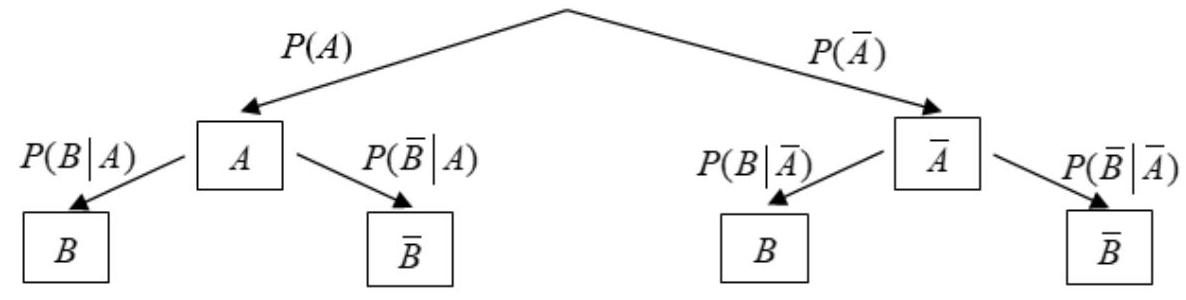
\includegraphics[width=\linewidth]{images/2025_01_02_562c5bc6077c0879a9a9g-2}

\section*{Definition}
Sei $(\Omega, P)$ ein diskreter Wahrscheinlichkeitsraum.\\
Zwei Ereignisse $A$ und $B$ heissen stochastisch unabhängig, falls gilt:

$$
P(A \cap B)=P(A) \cdot P(B)
$$

Andernfalls heissen $A$ und $B$ stochastisch abhängig.\\
Zwei Zufallsvariablen $X: \Omega \rightarrow \mathbb{R}$ und $Y: \Omega \rightarrow \mathbb{R}$ heissen stochastisch unabhängig, falls gilt:

$$
P(X=x, Y=y)=P(X=x) \cdot P(Y=y) \text { für alle } x, y \in \mathbb{R}
$$

Andernfalls heissen die Zufallsvariablen stochastisch abhängig.\\
Die Funktion $f(x, y)=P(X=x, Y=y)$ heisst die gemeinsame Verteilung (Verbundverteilung) von $X$ und $Y$.

\section*{Satz (Stochastische Unabhängigkeit)}
Sei $(\Omega, P)$ ein diskreter Wahrscheinlichkeitsraum.

\begin{itemize}
  \item Folgende Eigenschaften sind äquivalent:\\
(i) $A$ und $B$ sind stochastisch unabhängig.\\
(ii) $A$ und $\Omega \backslash B$ sind stochastisch unabhängig.\\
(iii) $\Omega \backslash A$ und $\Omega \backslash B$ sind stochastisch unabhängig.
  \item Wenn $A$ und $B$ stochastisch unabhängig sind, beeinflusst das Eintreten des einen Ereignisses das Eintreten des anderen Ereignisses nicht.\\
Denn falls $P(B) \neq 0$, so gilt $P(A \mid B)=P(A)$ und falls $P(A) \neq 0$, so gilt $P(B \mid A)=P(B)$.
  \item Für stochastisch unabhängige Zufallsvariablen $X$ und $Y$ gilt:
\end{itemize}

$$
E(X \cdot Y)=E(X) \cdot E(Y) \text { und } V(X+Y)=V(X)+V(Y)
$$

Zuletzt geändert: Mittwoch, 8. Dezember 2021, 11:13\\
3. Zusammenfassung: Kombinatorik

\section*{Direkt zu:}
\begin{enumerate}
  \setcounter{enumi}{4}
  \item Zusammenfassung: Spezielle Verteilungen
\end{enumerate}

\end{document}